\chapter{問題提起}
% Tanimu先輩"具体的に都市の画像を用いた想定している有効活用の方法について話す.軽く"
% 俺の研究の場合どんな問題について語ればいいんだろうねよくわからん
% 多分渋滞についての問題を書けばいいのかもしれない(適当)
ここでは本研究をするにあたって、本研究が意識する問題について述べる。

\section{渋滞}
% 渋滞情報はどのように作られるのか
% VICSの話
\subsection{渋滞検知}
現在の渋滞は主要な道路にセンサーやカメラなどを取り付けてリアルタイムに渋滞情報を検知し管理している。
渋滞情報の取得には一般財団法人道路交通情報通信システムセンター(VICS)が関わっている。
VICSではVICSセンターが国土交通省、地方自治体および都道府県警察からの渋滞情報を集めて管理している。
集められた渋滞情報はFM多重放送、電波ビーコン、光ビーコンといった道路に設置された通信機でVICS対応カーナビゲーションシステムに送信し、渋滞情報や目的地までの到着予想時刻としてドライバーが受け取っている。
また、特に高速道路における渋滞情報の取得については、道路に2km間隔でトラフィックカウンターという計測器が埋め込まれており、通過する車の台数、大型車や小型車の区別、車の速度を計測している。
トラフィックカウンターだけではなく、高速道路においては交通管理隊が常に巡回しており、渋滞を見つけると無線で交通管制センターへ連絡し、ドライバーへフィードバックしている(参照:\figref{fig:vics_system})。

\begin{figure}[htbp]
  \begin{center}
   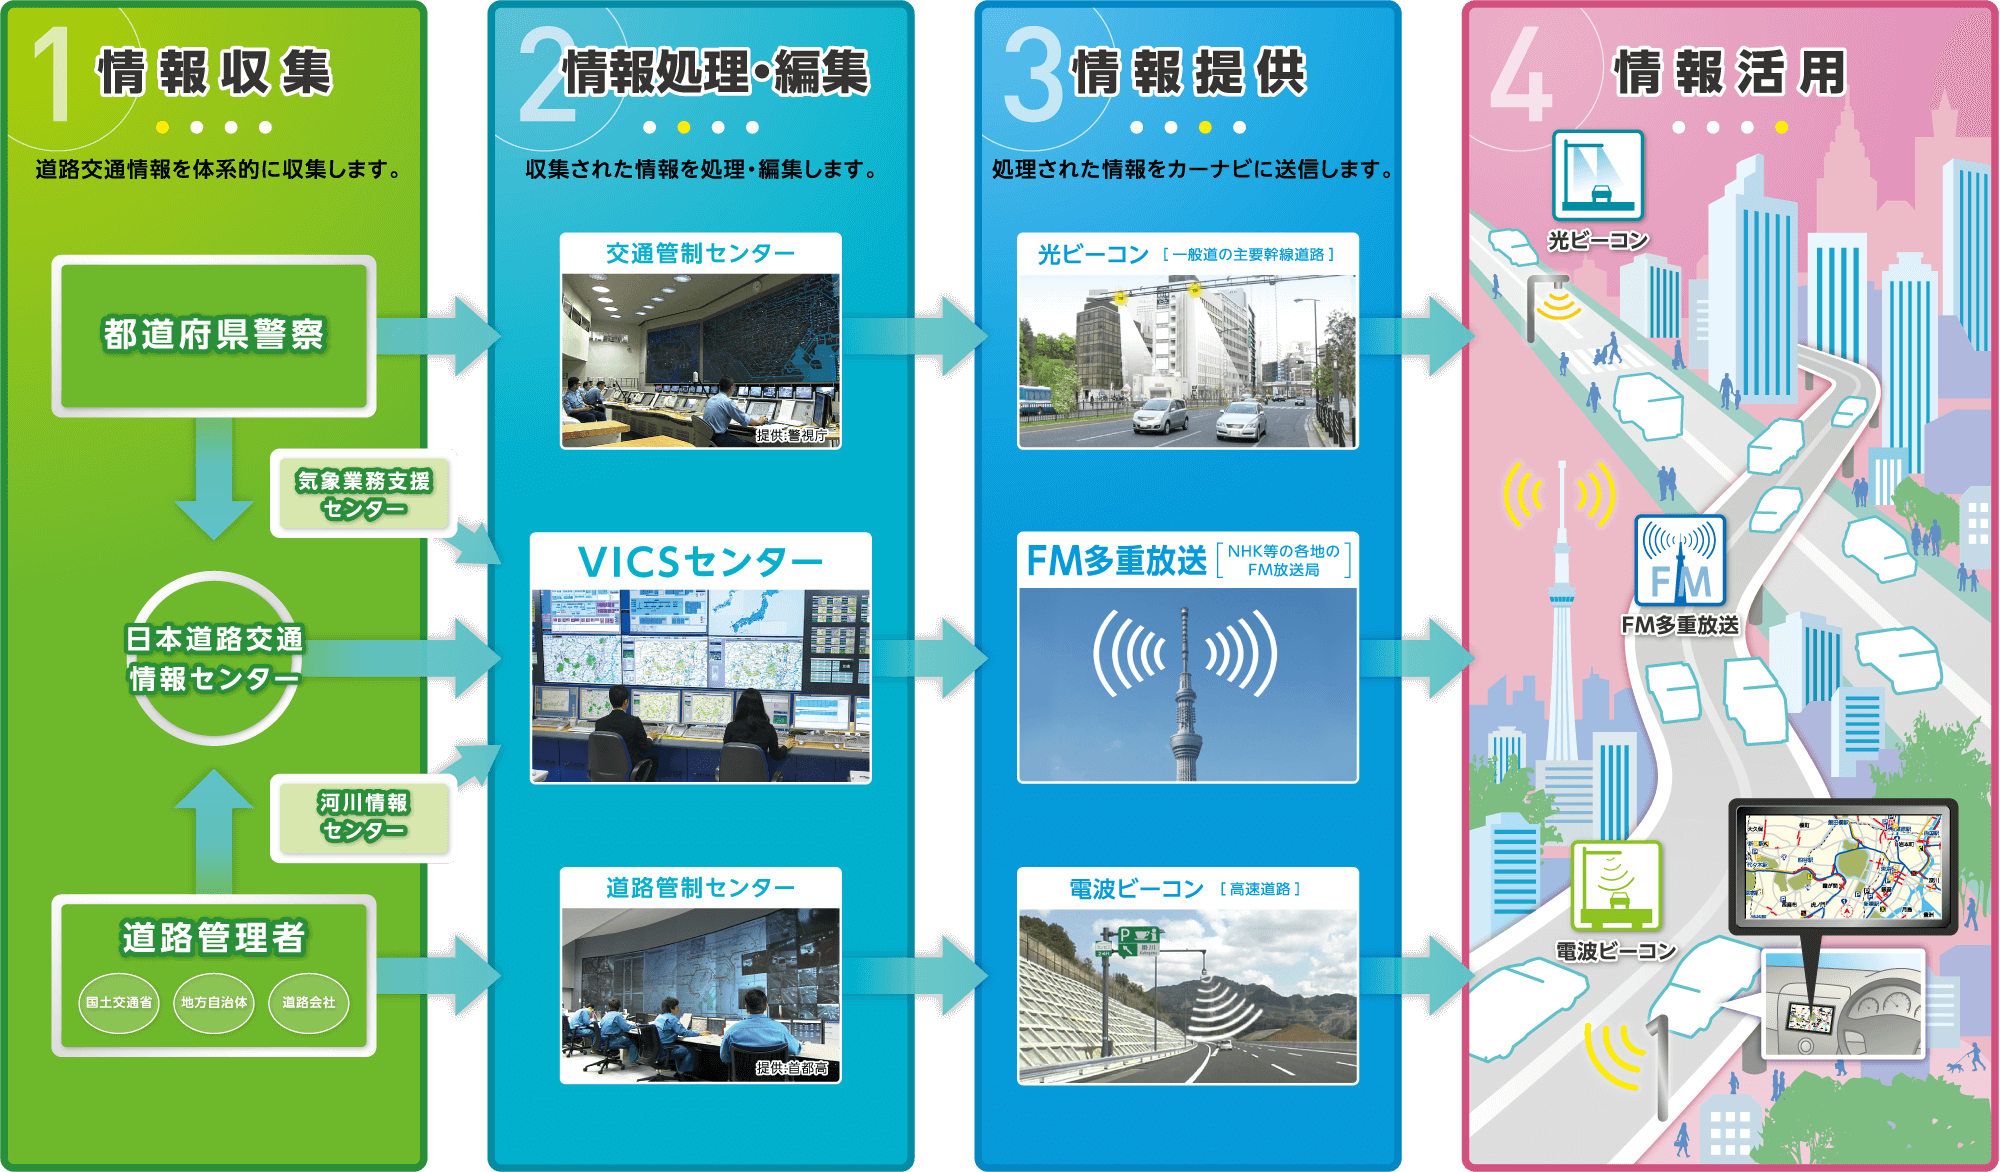
\includegraphics[width=11cm]{figs/vics.png}
  \end{center}
  \caption{VICSの仕組み(https://www.vics.or.jp/know/about/center.html)}
  \label{fig:vics_system}
\end{figure}

% それがどう不備なのか
しかし現状、渋滞情報は高速道路や国道といった主要な道路のみの情報しか得られておらず、それ以外の比較的小さい道路では渋滞情報を取得することができない問題がある。
例えば旅行シーズン中など、普段の走行量が少ない道路にて走行量が急に増えた際に、事前に渋滞情報を取得して迂回することが困難になる。
特に、1車線のような小さい道路が急な渋滞になるケースのことが多く、一度渋滞にはまってしまうと迂回ルートを取ろうとしても抜け出すことが難しくなる。

また、VICS非対応のカーナビゲーションが存在することも問題の一つである。
日本は世界的な自動車生産量を誇り、日本で走っている自動車はほとんどが国産車である。
しかし、2019年度の統計によると、日本市場における輸入車のシェアは6\%となっており、輸入車に載っている人口は一定数いることがわかる。
輸入車に乗っている人はVICS対応のカーナビゲーションを購入する必要がある。
また、日本で販売しているカーナビゲーションにもVICSに対応していない機種が存在する。

% プローブ情報を活用した例
\subsection{プローブ情報}
2020年よりVICSは渋滞ゼロ社会を目指すためにプローブ情報を利用したサービスの実証実験を行なっている(参照:\figref{fig:probe})。
プローブ情報とは、車一台一台の位置、速度、通過時刻等の等の走行軌跡データーを指す。
プローブ情報を活用することでこれまでトラフィックカウンターがなかった場所でも渋滞情報を取得することを目指し、実証実験を行なっている。

\begin{figure}[htbp]
  \begin{center}
   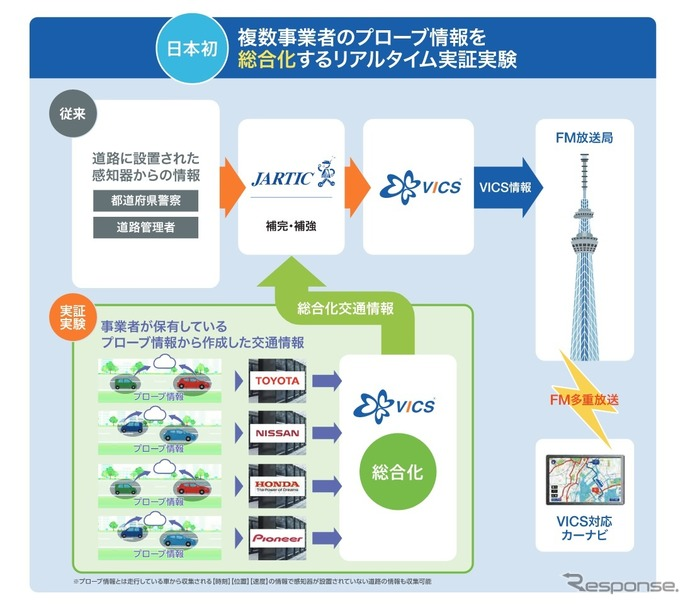
\includegraphics{figs/probe.jpg}
  \end{center}
  \caption{実証実験中のプローブ情報を利用したシステム(https://response.jp/article/2020/03/05/332331.html)}
  \label{fig:probe}
\end{figure}
\newpage
しかし、プローブ情報には車のセンサーを主に使っているため、ドライブレコーダーを使う等の情報はない。
センサーの情報のみを使って渋滞検知を行おうとすると、例えば低速運行しているのは渋滞に巻き込まれたからなのか、他の理由があるからなのか等の情報を得ることができない。
また、車が停止したのは渋滞のためなのか、停止信号のためなのか、あるいは駐車のためなのかといった情報もセンサーからのみでは得ることができない。
これらの情報を得るにあたって、ドライブレコーダーの使用は避けて通れないと考える。

% 渋滞に巻き込まれなくなることのメリットとか書いたほうがいいかな?

\section{ドライブレコーダー}
% ドライブレコーダーの問題点
次に、ドライブレコーダーについて述べる。
% ドライブレコーダーの搭載率
2020年1月に国道交通省が出した統計によると、統計対象者のうちドライブレコーダーを実際に取り付けている割合は45.9\%という結果が出た。